\documentclass[12pt, titlepage]{article}

\usepackage{fullpage}
\usepackage[round]{natbib}
\usepackage{multirow}
\usepackage{booktabs}
\usepackage{tabularx}
\usepackage{graphicx}
\usepackage{float}
\usepackage{hyperref}
\hypersetup{
    colorlinks,
    citecolor=blue,
    filecolor=black,
    linkcolor=red,
    urlcolor=blue
}

%% Comments

\usepackage{color}

\newif\ifcomments\commentstrue %displays comments
%\newif\ifcomments\commentsfalse %so that comments do not display

\ifcomments
\newcommand{\authornote}[3]{\textcolor{#1}{[#3 ---#2]}}
\newcommand{\todo}[1]{\textcolor{red}{[TODO: #1]}}
\else
\newcommand{\authornote}[3]{}
\newcommand{\todo}[1]{}
\fi

\newcommand{\wss}[1]{\authornote{blue}{SS}{#1}} 
\newcommand{\plt}[1]{\authornote{magenta}{TPLT}{#1}} %For explanation of the template
\newcommand{\an}[1]{\authornote{cyan}{Author}{#1}}

%% Common Parts

\newcommand{\progname}{Mechatronics} % PUT YOUR PROGRAM NAME HERE
\newcommand{\authname}{Team \#20, Team Name
\\ Robert Zhu zhul49
\\ Zifan Meng mengz17
\\ Jiahui Chen chenj194
\\ Kelvin Huynh huynhk12
\\ Runze Zhu zhur25
\\ Mirza Nafi Hasan hasanm21} % AUTHOR NAMES                  

\usepackage{hyperref}
    \hypersetup{colorlinks=true, linkcolor=blue, citecolor=blue, filecolor=blue,
                urlcolor=blue, unicode=false}
    \urlstyle{same}
                                


\newcounter{acnum}
\newcommand{\actheacnum}{AC\theacnum}
\newcommand{\acref}[1]{AC\ref{#1}}

\newcounter{ucnum}
\newcommand{\uctheucnum}{UC\theucnum}
\newcommand{\uref}[1]{UC\ref{#1}}

\newcounter{mnum}
\newcommand{\mthemnum}{M\themnum}
\newcommand{\mref}[1]{M\ref{#1}}

\begin{document}

\title{Module Guide for \progname{}} 
\author{\authname}
\date{\today}

\maketitle

\pagenumbering{roman}

\section{Revision History}

\begin{tabularx}{\textwidth}{p{3cm}p{2cm}X}
\toprule {\bf Date} & {\bf Version} & {\bf Notes}\\
\midrule
January 18, 2023 & 1.0 & Everyone - Initial MG Draft\\
\bottomrule
\end{tabularx}

\newpage

\section{Reference Material}

This section records information for easy reference.

\subsection{Abbreviations and Acronyms}

\renewcommand{\arraystretch}{1.2}
\begin{tabular}{l l} 
  \toprule		
  \textbf{symbol} & \textbf{description}\\
  \midrule 
  AC & Anticipated Change\\
  DAG & Directed Acyclic Graph \\
  M & Module \\
  MG & Module Guide \\
  OS & Operating System \\
  R & Requirement\\
  SC & Scientific Computing \\
  SRS & Software Requirements Specification\\
  \progname & Explanation of program name\\
  UC & Unlikely Change \\
  \bottomrule
\end{tabular}\\

\newpage

\tableofcontents

\listoftables

\listoffigures

\newpage

\pagenumbering{arabic}

\section{Introduction}

Decomposing a system into modules is a commonly accepted approach to developing
software.  A module is a work assignment for a programmer or programming
team~\citep{ParnasEtAl1984}.  We advocate a decomposition
based on the principle of information hiding~\citep{Parnas1972a}.  This
principle supports design for change, because the ``secrets'' that each module
hides represent likely future changes.  Design for change is valuable in SC,
where modifications are frequent, especially during initial development as the
solution space is explored.  

Our design follows the rules layed out by \citet{ParnasEtAl1984}, as follows:
\begin{itemize}
\item System details that are likely to change independently should be the
  secrets of separate modules.
\item Each data structure is implemented in only one module.
\item Any other program that requires information stored in a module's data
  structures must obtain it by calling access programs belonging to that module.
\end{itemize}

After completing the first stage of the design, the Software Requirements
Specification (SRS), the Module Guide (MG) is developed~\citep{ParnasEtAl1984}. The MG
specifies the modular structure of the system and is intended to allow both
designers and maintainers to easily identify the parts of the software.  The
potential readers of this document are as follows:

\begin{itemize}
\item New project members: This document can be a guide for a new project member
  to easily understand the overall structure and quickly find the
  relevant modules they are searching for.
\item Maintainers: The hierarchical structure of the module guide improves the
  maintainers' understanding when they need to make changes to the system. It is
  important for a maintainer to update the relevant sections of the document
  after changes have been made.
\item Designers: Once the module guide has been written, it can be used to
  check for consistency, feasibility and flexibility. Designers can verify the
  system in various ways, such as consistency among modules, feasibility of the
  decomposition, and flexibility of the design.
\end{itemize}

The rest of the document is organized as follows. Section
\ref{SecChange} lists the anticipated and unlikely changes of the software
requirements. Section \ref{SecMH} summarizes the module decomposition that
was constructed according to the likely changes. Section \ref{SecConnection}
specifies the connections between the software requirements and the
modules. Section \ref{SecMD} gives a detailed description of the
modules. Section \ref{SecTM} includes two traceability matrices. One checks
the completeness of the design against the requirements provided in the SRS. The
other shows the relation between anticipated changes and the modules. Section
\ref{SecUse} describes the use relation between modules.

\section{Anticipated and Unlikely Changes} \label{SecChange}

This section lists possible changes to the system. According to the likeliness
of the change, the possible changes are classified into two
categories. Anticipated changes are listed in Section \ref{SecAchange}, and
unlikely changes are listed in Section \ref{SecUchange}.

\subsection{Anticipated Changes} \label{SecAchange}

Anticipated changes are the source of the information that is to be hidden
inside the modules. Ideally, changing one of the anticipated changes will only
require changing the one module that hides the associated decision. The approach
adapted here is called design for
change.

\begin{description}
\item[\refstepcounter{acnum} \actheacnum \label{acMotionT}:] The implementation of a more advanced motion tracking algorithm so that continuous motions with faster speed can be captured.
\item[\refstepcounter{acnum} \actheacnum \label{acCoordN}:] The formatting of the normalized coordinates input into the Classification Module.
\item[\refstepcounter{acnum} \actheacnum \label{acCoordE}:] The format of export normalized coordinates.
\item[\refstepcounter{acnum} \actheacnum \label{acVideoC}:] Allow for static image input to enable training using larger datasets.
\item[\refstepcounter{acnum} \actheacnum \label{acVideoA}:] Increase the area that the recognition boundary encloses for recognizing more complicated gestures.
\item[\refstepcounter{acnum} \actheacnum \label{acKeyPointC}:] Modify keypoint classification to check multiple points instead of single point for more complex motion.
\item[\refstepcounter{acnum} \actheacnum \label{acML}:] Change from static classifier set to a dynamic classifier set that is able to expand the number of gestures.
\item[\refstepcounter{acnum} \actheacnum \label{acTraining}:] The implementation of a more suitable machine learning model for better performance.
\item[\refstepcounter{acnum} \actheacnum \label{acTextToSpeech}:] The implementation of reading a translated script into audio output through Raspberry Pi.
\item[\refstepcounter{acnum} \actheacnum \label{acHardware}:] The hardware tracking devices on which the the software is running was replaced with a Raspberry Pi with the camera from a PC.



\end{description}

\subsection{Unlikely Changes} \label{SecUchange}

The module design should be as general as possible. However, a general system is
more complex. Sometimes this complexity is not necessary. Fixing some design
decisions at the system architecture stage can simplify the software design. If
these decision should later need to be changed, then many parts of the design
will potentially need to be modified. Hence, it is not intended that these
decisions will be changed.

\begin{description}
\item[\refstepcounter{ucnum} \uctheucnum \label{uc1}:] The csv format to another file type.
\item[\refstepcounter{ucnum} \uctheucnum \label{uc2}:] The output to just TTS instead of both TTS and video.
\item[\refstepcounter{ucnum} \uctheucnum \label{uc3}:] Capture full body and facial recognition for sign language.
\item[\refstepcounter{ucnum} \uctheucnum \label{uc4}:] The hardware design is not likely to change once it is finished.
\item[\refstepcounter{ucnum} \uctheucnum \label{uc5}:] Training method for the machine learning model.
\item[\refstepcounter{ucnum} \uctheucnum \label{uc6}:] The goal for the ASL translator is to translate the user’s hand gestures to the corresponding English words or phrases.
\end{description}

\section{Module Hierarchy} \label{SecMH}

This section provides an overview of the module design. Modules are summarized
in a hierarchy decomposed by secrets in Table \ref{TblMH}. The modules listed
below, which are leaves in the hierarchy tree, are the modules that will
actually be implemented.

\begin{description}
\item [\refstepcounter{mnum} \mthemnum \label{m1}:] Motion Tracking Module
\item [\refstepcounter{mnum} \mthemnum \label{m2}:] Coordinate Normalization Module
\item [\refstepcounter{mnum} \mthemnum \label{m3}:] Coordinate Export Module
\item [\refstepcounter{mnum} \mthemnum \label{m4}:] Video Capture Module
\item [\refstepcounter{mnum} \mthemnum \label{m5}:] Video Analysis Module
\item [\refstepcounter{mnum} \mthemnum \label{m6}:] Key Point Classification Module
\item [\refstepcounter{mnum} \mthemnum \label{m7}:] Machine Learning Modules
\item [\refstepcounter{mnum} \mthemnum \label{m8}:] Training Module
\item [\refstepcounter{mnum} \mthemnum \label{m9}:] Text-to-Speech Module
\item [\refstepcounter{mnum} \mthemnum \label{m10}:] Hardware Hiding Module
\end{description}

\begin{table}[h!]
\centering
\begin{tabular}{p{0.3\textwidth} p{0.6\textwidth}}
\toprule
\textbf{Level 1} & \textbf{Level 2}\\
\midrule
{Hardware-Hiding Module} & Video Capture Module \\
\midrule
\multirow{7}{0.3\textwidth}{Behaviour-Hiding Module} & Text-to-Speech Module\\
& Key Point Classification Module - Communicates with ML module with data from coordinate normalization module\\
& Training Module - Communicates with ML module to update dataset\\
& Coordinate Export Module - Read data from video capture and stores into file\\
& Motion Tracking Module - Controller (ties everything together)\\
\midrule
\multirow{3}{0.3\textwidth}{Software Decision Module} & Video Analysis Module - requires data to be used\\
& Machine Learning Module\\
& Coordinate Normalization Module\\
\bottomrule
\end{tabular}
\caption{Module Hierarchy}
\label{TblMH}
\end{table}

\newpage

\section{Connection Between Requirements and Design} \label{SecConnection}

The design of the system is intended to satisfy the requirements developed in
the SRS. In this stage, the system is decomposed into modules. The connection
between requirements and modules is listed in Table \ref{TblRT}.

\section{Module Decomposition} \label{SecMD}

\subsection{Hardware Hiding Modules (\mref{m10})}

\begin{description}
  \item[Secrets:] The data structure and algorithm used to implement the virtual hardware
  \item[Services:] Serves as a virtual hardware used by the rest of the system. This module provides the interface between the hardware and the software. So, the system can use it to display outputs or to accept inputs
  \item[Implemented By:] OS
  \end{description}
  
\subsubsection{Video Capture Module (\mref{m4})}

\begin{description}
  \item[Secrets:] The algorithm used to track hand movement through any camera lens
  \item[Services:] Allows the progrom to interface with an external recording devices
  \item[Implemented By:] TensorFlow
  \end{description}

\subsection{Behaviour-Hiding Module}

\subsubsection{Key-Point Classification Module (\mref{m6})}

\begin{description}
  \item[Secrets:] The algorithm used to return index/classifier closest to the normalized coordinates
  \item[Services:] Provides communication between the motion tracking module and the machine learning module by storing the gathered information in the dataset
  \item[Implemented By:] Python
  \end{description}

\subsubsection{Text-to-Speech Module (\mref{m4})}

\begin{description}
  \item[Secrets:] The algorithm and dataset used to translate text-to-speech
  \item[Services:] This module serves as the method by which the sign language gesture will be converted into audio output
  \item[Implemented By:] Python
  \end{description}  
  
\subsubsection{Training Module (\mref{m8})}

\begin{description}
  \item[Secrets:] Gathers data points from the user and formats the structure into input for machine learning
  \item[Services:] Combines classifier label and coordinate data for application use
  \item[Implemented By:] Python
  \end{description}
  


\subsubsection{Coordinate Export Module (\mref{m3})}
\begin{description}
  \item[Secrets:] The algorithm used to create a dataset for the machine learning model
  \item[Services:] Provides access to normalized coordinate data
  \item[Implemented By:] Python
  \end{description}
  


\subsubsection{Motion Tracking Module (\mref{m1})}

\begin{description}
  \item[Secrets:] The algorithm by which the software detects the hand gestures performed in ASL
  \item[Services:] Receives the video from the camera as input, and locates the different hand joints to return the coordinates of the hand position
  \item[Implemented By:] Python
  \end{description}
  


\subsection{Software Decision Module}

\subsubsection{Machine Learning Module (\mref{m7})}

\begin{description}
  \item[Secrets:] The data structure in which classifier label data is paired with normalized coordinate data
  \item[Services:] Automates classification of sign language based on input coordinate data
  \item[Implemented By:] Python
  \end{description}
  

\subsubsection{Video Analysis Module (\mref{m5})}

\begin{description}
  \item[Secrets:] The algorithm by which the hand joints and classifier are displayed for the user
  \item[Services:] Based on the data from the Motion Tracking Module (M1), the algorithm places a joint overlay over the user’s hand as a visual tracker for all 20 joints
  \item[Implemented By:] Python
  \end{description}
  

\subsubsection{Coordinate Normalization Module (\mref{m2})}

\begin{description}
  \item[Secrets:] The algorithm to restructure the coordinates gathered from users into a value between 1 and -1
  \item[Services:] Standardizes the coordinate data allowing for different resolutions in cameras to be used
  \item[Implemented By:] Python
  \end{description}
  

\section{Traceability Matrix} \label{SecTM}

This section shows two traceability matrices: between the modules and the
requirements and between the modules and the anticipated changes.

% the table should use mref, the requirements should be named, use something
% like fref
\begin{table}[H]
\centering
\begin{tabular}{p{0.2\textwidth} p{0.6\textwidth}}
\toprule
\textbf{Req.} & \textbf{Modules}\\
\midrule
CFR1 & \mref{m1}, \mref{m4}\\
CFR2 & \mref{m5}\\
MLFR1 & \mref{m2}\\
MLFR2 & \mref{m3}\\
MLFR3 & \mref{m4}\\
MLFR4 & \mref{m6}, \mref{m9}, \mref{m10}\\
MLFR5 & \mref{m4}\\
MLFR6 & \mref{m4}\\
MLFR7 & \mref{m7}, \mref{m8}\\
NFR1 & \mref{m5}, \mref{m6}, \mref{m7}\\
NFR2 & \mref{m1}, \mref{m4}\\
NFR3 & \mref{m9}\\
NFR4 & \mref{m9}\\
NFR5 & \mref{m7}\\
NFR6 & \mref{m10}\\
NFR7 & \mref{m1}, \mref{m4}, \mref{m9}\\

\bottomrule
\end{tabular}
\caption{Trace Between Requirements and Modules}
\label{TblRT}
\end{table}

\begin{table}[H]
\centering
\begin{tabular}{p{0.2\textwidth} p{0.6\textwidth}}
\toprule
\textbf{AC} & \textbf{Modules}\\
\midrule
\acref{acMotionT} & \mref{m1}\\
\acref{acCoordN} & \mref{m2}\\
\acref{acCoordE} & \mref{m3}\\
\acref{acVideoC} & \mref{m4}\\
\acref{acVideoA} & \mref{m5}\\
\acref{acKeyPointC} & \mref{m6}\\
\acref{acML} & \mref{m7}\\
\acref{acTraining} & \mref{m8}\\
\acref{acTextToSpeech} & \mref{m9}\\
\acref{acHardware} & \mref{m10}\\





\bottomrule
\end{tabular}
\caption{Trace Between Anticipated Changes and Modules}
\label{TblACT}
\end{table}

\section{Use Hierarchy Between Modules} \label{SecUse}

In this section, the uses hierarchy between modules is
provided. \citet{Parnas1978} said of two programs A and B that A {\em uses} B if
correct execution of B may be necessary for A to complete the task described in
its specification. That is, A {\em uses} B if there exist situations in which
the correct functioning of A depends upon the availability of a correct
implementation of B.  Figure \ref{FigUH} illustrates the use relation between
the modules. It can be seen that the graph is a directed acyclic graph
(DAG). Each level of the hierarchy offers a testable and usable subset of the
system, and modules in the higher level of the hierarchy are essentially simpler
because they use modules from the lower levels.

\begin{figure}[H]
\centering
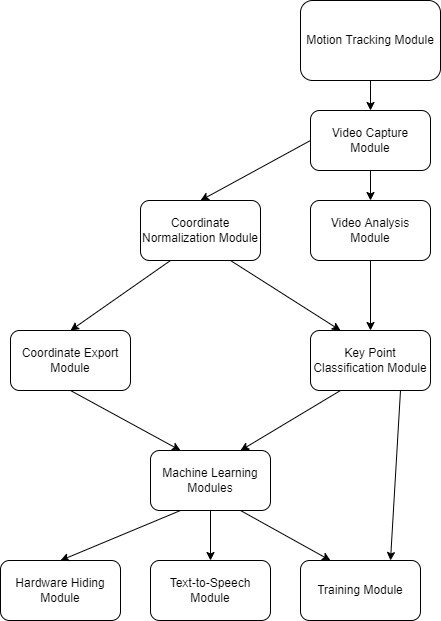
\includegraphics[width=0.7\textwidth]{Hierarchy.jpg}
\caption{Use hierarchy among modules}
\label{FigUH}
\end{figure}

%\section*{References}

\bibliographystyle {plainnat}
\bibliography{../../../refs/References}

\end{document}
